\section{Gestion et déroulement du projet}

    \subsection{Planning}

        \begin{frame}
            \frametitle{Planning prévisionnel}
            \centering{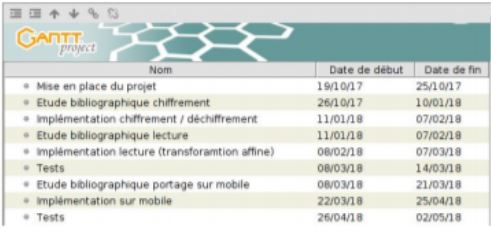
\includegraphics[width=.8\linewidth]{./rsc/gant_1_1.png}}
            \centering{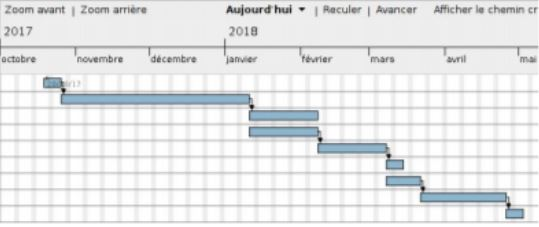
\includegraphics[width=.8\linewidth]{./rsc/gant_1_2.png}}
        \end{frame}

        \begin{frame}
            \frametitle{Planning final}
            \centering{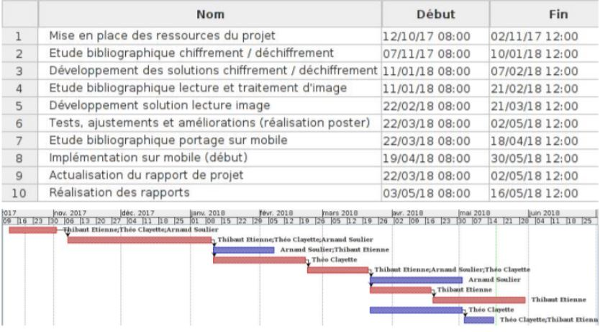
\includegraphics[width=\linewidth]{./rsc/gant_2.png}}
        \end{frame}

    \subsection{Données quantitatives}

        \begin{frame}
            \frametitle{Commit}
            \centering{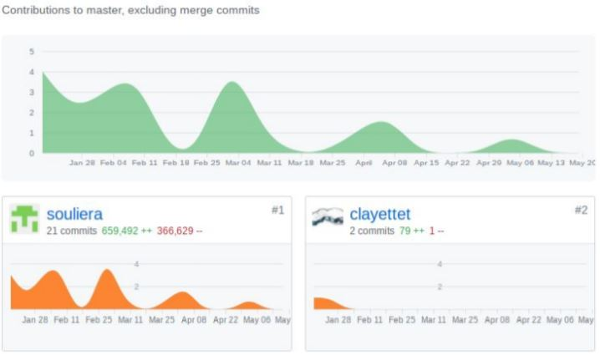
\includegraphics[width=.8\linewidth]{./rsc/commit.png}}
            \begin{exampleblock}{Observations}
                \begin{itemize}
                    \item Constant sur l'ensemble du projet (pas de rush final).
                    \item Développement en extrem programming.
                    \item Push avec un seul compte pour éviter les merges.
                \end{itemize}
            \end{exampleblock}
        \end{frame}

        \begin{frame}
            \frametitle{Nombre de ligne de code}
            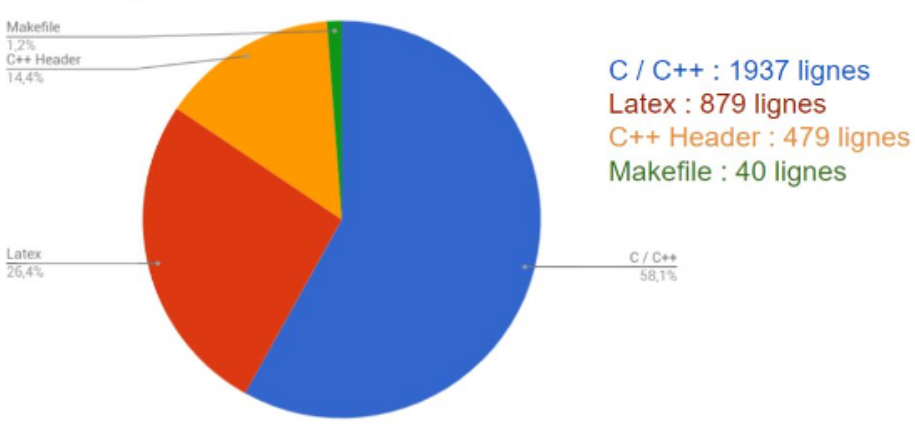
\includegraphics[width=\linewidth]{./rsc/lignes_code.png}
        \end{frame}

    \subsection{Analyse du risque}

        \begin{frame}
            \frametitle{Analyse du risque}
            \centering{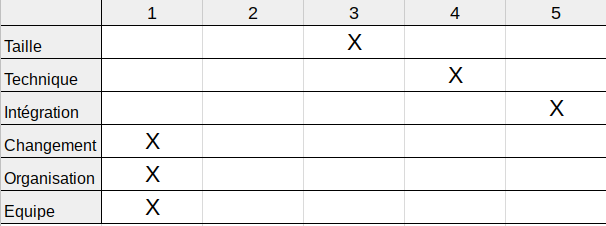
\includegraphics[width=\linewidth]{./rsc/risque.png}}
        \end{frame}

    \subsection{Problèmes et suite}

        \begin{frame}
            \frametitle{Problèmes rencontrés}
            \begin{block}{Github}
                Extrem Programming et push avec un seul compte.
            \end{block}
            \begin{block}{Équilibre entre qualité et temps de calcul}
                Mesure du Peak Signal to Noise Ratio (PSNR).
            \end{block}
            \begin{block}{Variation des résultats en fonction de l'éclairage ambiant}
                Correction de la balance des blancs.
            \end{block}
        \end{frame}

        \begin{frame}
            \frametitle{Features en cours}
            \begin{block}{Features en cours}
                \begin{itemize}
                    \item Portage sur mobile.
                    \item Portage sur de la vidéo.
                    \item Portage sur une application "en direct" permettant le sur-impression de l'oeuvre déchiffrée sur l'oeuvre chiffrée par simple pointage de l'appareil photo sur la cible.
                    \item Portage de la fonctionnalité précédente sur un casque de réalité augmentée.
                \end{itemize}
            \end{block}
        \end{frame}
